
This section outlines broadcast communication abstractions, utilized in \nameNS, under the unique environment of a fully connected network. 
While by Sec.~\ref{section_model} nodes in the network are assumed to be fully connected, a forwarding scheme determines which of the links to use to optimize a relevant metric. We refer to the node who starts disseminating a message as the message originator. 
We describe two high level approaches for communication. The first aims to reduce dissemination time, while the second aims to maximize originator anonymity. 
We start with some notations and intuition.
% Use case - guaranteed fast dissemination	time - propagate EB+BP, Block Shares - the creation of each new block is reliant on the previous decrypted block - the propagation time of the mentioned information will affect the throughput.  
% as each decrypted block dictates the 2 provide both 
% Second, the timouts used in PBFT are derived from the bound on this propagation time - 




%Motivation + use case for each method

% The anonymity protocol is used to propagate the encrypted transaction. To maintain representation fairness (Sec. ?), transactions are not only encrypted, but also hide their originator node.  
% Mixnets for anonymity

%We realize them in multiple suggested forwarding schemes.
%%When and why we use each approach/    
\subsection{Background}
%settings (n,f,k)
% Working in a coordinated manner as a whole, depends on the components ability to disseminate information. Interactions between processes should manifest desired qualities, as speed or reliability. 
The design of a forwarding scheme can influence several performance metrics such as:

\begin{enumerate}
\item The dissemination time of a message.
\item The required fan-out of a node number, describing the maximal amount of message copies required to be sent by a node.
\item Resistance to faulty nodes which, for instance, unexpectedly do not forward messages.
\item Various privacy aspects, e.g., the anonymity of the message source. 
%Anonymity can be measured, for instance, by the ratio of potential senders of a message among all nodes. 
\end{enumerate}
Often, there is a tradeoff between these metrics, such that one can be improved only at the expense of some others. 


Consider for instance the  basic forwarding schemes illustrated in Fig.~\ref{fig_basic_routing} and assume all links share the same propagation delay. First, in Fig.~\ref{fig_basic_routing_a}, a message is sent from its source directly to all other nodes along their connecting link. Accordingly, all nodes receive the message within a single hop time, achieving an ideal dissemination time.  On the other hand, when a node receives a message, she immediately  knows the identity of its originator. This is the node from which the message was received.  This implies a complete avoidance of originator anonymity. 

In the scheme of Fig.~\ref{fig_basic_routing_b}, a message is forwarded as in a ring such that each node transmits messages only to a single node, the following node in some predetermined order of the nodes. Here, it might take a node several hops to receive a message where the exact time it takes  is determined by her location with regards to the source location such that the maximal delay is $n-1$ hops for $n$ connected nodes. 
%The scheme is not tolerant to the existence of Byzantine nodes that the existence of even one of them can eliminate nodes from receiving a message. 
Likewise,  the scheme of Fig.~\ref{fig_basic_routing_c} tries to balance these two metrics. A message is first sent to a common central node that forwards it to all other nodes. A message has a fixed delay of two hops and a node always receives a message from the central node without revealing an information regarding the originator. Note that here, the central node does know the originator identity. Moreover, operation highly relies on the assumption that the central node follows her expected behavior. 

%Accordingly, our solution relies on more than a single forwarding scheme suggested for various message types.
In the analysis of the  described forwarding schemes we make use of parameters such as $n$, $f$ and $k$. $n$ describes the total number of network nodes forwarding and receiving messages. Among these  at most $f$ are Byzantine, and no node transmits a message to more than $k$ of her neighbors. 
From bandwidth considerations we want to keep $k$ small, while it is quite clear $k<f$ cannot allow dealing with $f$ Byzantine nodes.

\begin{figure}[!b]%[!ht]
	\centering
	\subfigure[Clique  forwarding] {
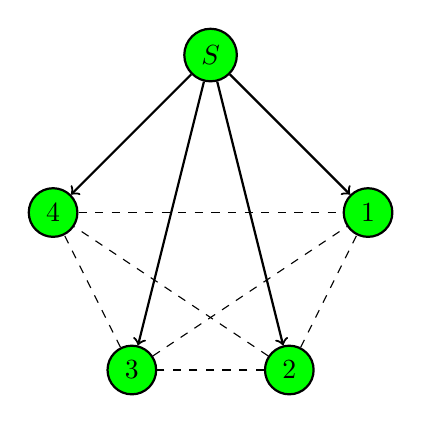
\begin{tikzpicture}
\tikzstyle{every loop}=[]
\node[style={circle,draw,thick,align=center, fill={green}}] (2) 
at (1, 0) {$3$};
\node[style={circle,draw,thick,align=center, fill={green}}] (3) at (0, 2) {$4$};
\node[style={circle,draw,thick,align=center, fill={green}}] (4) at (2, 4) {$S$};
\node[style={circle,draw,thick,align=center, fill={green}}] (5) at (4, 2) {$1$};
\node[style={circle,draw,thick,align=center, fill={green}}] (1) at (3, 0) {$2$};
\path[]
    (1) [-,dashed] edge node[above,minimum size=0pt] {} (2)
    (1) [-,dashed] edge node[above,minimum size=0pt] {} (3)
    (1) [-,dashed] edge node[above,minimum size=0pt] {} (5)
    (2) [-,dashed] edge node[above,minimum size=0pt] {} (3)
    (2) [-,dashed] edge node[above,minimum size=0pt] {} (5)
    (3) [-,dashed] edge node[below,minimum size=0pt] {} (5);
\path[]
    (4) [->,solid,thick] edge node[right,minimum size=0pt] {} (1)
    (4) [->,solid,thick] edge node[right,minimum size=0pt] {} (2)
    (4) [->,solid,thick] edge node[right,minimum size=0pt] {} (3)
    (4) [->,solid,thick] edge node[right,minimum size=0pt] {} (5);
\end{tikzpicture}
		\label{fig_basic_routing_a}
	}
%\hspace{5pt}
	\subfigure[Ring  forwarding] {
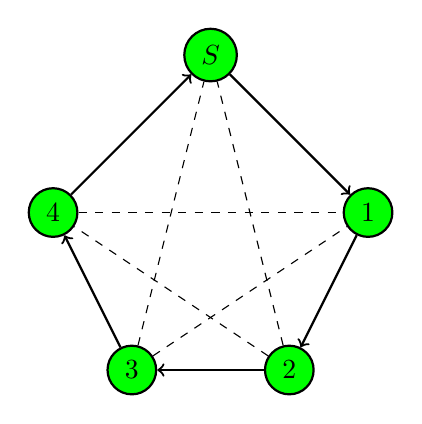
\begin{tikzpicture}
\tikzstyle{every loop}=[]
\node[style={circle,draw,thick,align=center, fill={green}}] (2) 
at (1, 0) {$3$};
\node[style={circle,draw,thick,align=center, fill={green}}] (3) at (0, 2) {$4$};
\node[style={circle,draw,thick,align=center, fill={green}}] (4) at (2, 4) {$S$};
\node[style={circle,draw,thick,align=center, fill={green}}] (5) at (4, 2) {$1$};
\node[style={circle,draw,thick,align=center, fill={green}}] (1) at (3, 0) {$2$};
\path[]
    (1) [-,dashed] edge node[above,minimum size=0pt] {} (3)
    (1) [-,dashed] edge node[above,minimum size=0pt] {} (4)
    (2) [-,dashed] edge node[above,minimum size=0pt] {} (4)
    (2) [-,dashed] edge node[above,minimum size=0pt] {} (5)
    (3) [-,dashed] edge node[below,minimum size=0pt] {} (5);
\path[]
    (1) [->,solid,thick] edge node[right,minimum size=0pt] {} (2)
    (2) [->,solid,thick] edge node[right,minimum size=0pt] {} (3)
    (3) [->,solid,thick] edge node[right,minimum size=0pt] {} (4)
    (4) [->,solid,thick] edge node[right,minimum size=0pt] {} (5)
    (5) [->,solid,thick] edge node[right,minimum size=0pt] {} (1);
\end{tikzpicture}
		\label{fig_basic_routing_b}
	}
    %\hspace{5pt}
	\subfigure[Star forwarding] {
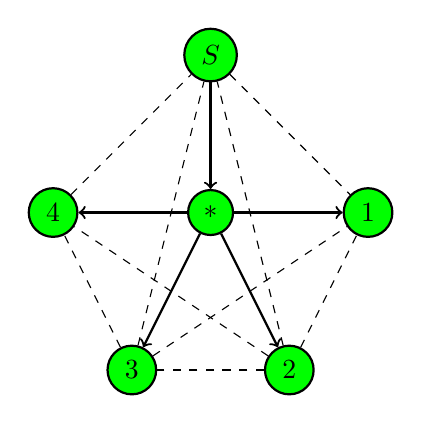
\begin{tikzpicture}
\tikzstyle{every loop}=[]
\node[style={circle,draw,thick,align=center, fill={green}}] (2) 
at (1, 0) {$3$};
\node[style={circle,draw,thick,align=center, fill={green}}] (3) at (0, 2) {$4$};
\node[style={circle,draw,thick,align=center, fill={green}}] (4) at (2, 4) {$S$};
\node[style={circle,draw,thick,align=center, fill={green}}] (5) at (4, 2) {$1$};
\node[style={circle,draw,thick,align=center, fill={green}}] (1) at (3, 0) {$2$};
\node[style={circle,draw,thick,align=center, fill={green}}] (6) at (2, 2) {$*$};
\path[]
	(1) [-,dashed] edge node[above,minimum size=0pt] {} (2)
    (1) [-,dashed] edge node[above,minimum size=0pt] {} (3)
    (1) [-,dashed] edge node[above,minimum size=0pt] {} (4)
    (1) [-,dashed] edge node[above,minimum size=0pt] {} (5)
    (2) [-,dashed] edge node[above,minimum size=0pt] {} (3)
%    (2) [-,dashed] edge node[above,minimum size=0pt] {} (4)
    (2) [-,dashed] edge node[above,minimum size=0pt] {} (5)
    (3) [-,dashed] edge node[below,minimum size=0pt] {} (4)
    (2) [-,dashed] edge node[below,minimum size=0pt] {} (4)
    (3) [-,dashed] edge node[below,minimum size=0pt] {} (6)
    (4) [-,dashed] edge node[below,minimum size=0pt] {} (5);
\path[]
	(4) [->,solid,thick] edge node[right,minimum size=0pt] {} (6)
    (6) [->,solid,thick] edge node[right,minimum size=0pt] {} (2)
    (6) [->,solid,thick] edge node[right,minimum size=0pt] {} (3)
    (6) [->,solid,thick] edge node[right,minimum size=0pt] {} (5)
    (6) [->,solid,thick] edge node[right,minimum size=0pt] {} (1);
\end{tikzpicture}
		\label{fig_basic_routing_c}
	}
	\\ \caption{Illustration of  various forwarding schemes. A message is transmitted from a source node $S$ to all other nodes, either directly or through intermediate nodes. 
	}\label{fig_basic_routing}
\end{figure}
%######## Model in the context of communication ##########
%%% network  - nodes..
%%% static byzantine
%%% arbitrary faults - deviate in any conceivable way
%%% limiting assumption - authenticated perfect links
%%% Timing assumption - links sync - bounded latency 
%%% property - Messages are self-verifiable\ relying on byzantine quorums (block proof, encrypted txs, block share) 
%%% Together with auth links - limits the adversary manipulation power - mainly to routing (where crash is routing 0)
% • (Purely asynchronous network) We assume each pair of nodes
% is connected by a reliable authenticated point-to-point channel
% that does not drop messages.2 The delivery schedule is entirely
% determined by the adversary, but every message sent between
% correct nodes must eventually be delivered. We will be interested
% in characterizing the running time of protocols based on the
% 2Reliable channels can be emulated on top of unreliable channels
% by resending transmissions, at the expense of some efficiency.
% number of asynchronous rounds (as described in Section 2). As
% the network may queue messages with arbitrary delay, we also
% assume nodes have unbounded buffers and are able to process all
% the messages they receive.
% • (Static Byzantine faults) The adversary is given complete control
% of up to f faulty nodes, where f is a protocol parameter. Note
% that 3 f +1 ≤ N (which our protocol achieves) is the lower bound
% for broadcast protocols in this setting.

%\subsection{System model}
\subsection{Minimizing worst-case dissemination time}
We focus here on the design of a forwarding scheme with \emph{a small worst-case delay}. In that, we refer to the maximal time it takes to send a message between any pair of source and destination nodes. We maintain the settings of $n$ nodes with $f$ Byzantines. %, while neglecting issues related to originator anonymity.
Denote by $\zeta$ the worst-case message delay, as a function of the number of hops.
Schemes are characterized by two parameters: the fan-out bound $k$  and the obtained delay $\zeta$. Intuitively, increasing the fan-out enables faster message dissemination. 
We describe forwarding schemes which illustrate this tradeoff. In the first scheme, the fan-out $k = O(\sqrt{n \cdot f})$ and the achieved delay is constant $\zeta=2$. In the second scheme $k=2 \cdot (f+1)$ and the achieved delay is $\zeta = O(\log({n/f}))$.


\begin{figure}[!b]%[!ht]
	\centering
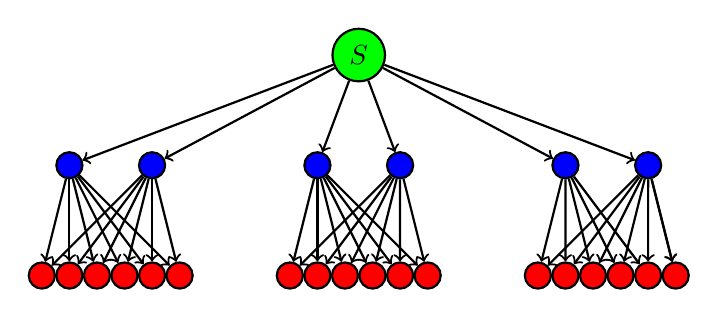
\begin{tikzpicture}[scale=0.7]
\tikzstyle{every loop}=[]
\node[style={circle,draw,thick,align=center, fill={green}}] (0) at (5.25, 4) {$S$};
\node[style={circle,draw,thick,align=center, fill={blue}}] (1) at (0, 2) {};
\node[style={circle,draw,thick,align=center, fill={blue}}] (2) at (1.5, 2) {};
\node[style={circle,draw,thick,align=center, fill={blue}}] (3) at (4.5, 2) {};
\node[style={circle,draw,thick,align=center, fill={blue}}] (4) at (6, 2) {};

\node[style={circle,draw,thick,align=center, fill={blue}}] (5) at (9, 2) {};
\node[style={circle,draw,thick,align=center, fill={blue}}] (6) at (10.5, 2) {};
\node[style={circle,draw,thick,align=center, fill={red}}] (11) at (-0.5, 0) {};
\node[style={circle,draw,thick,align=center, fill={red}}] (12) at (0, 0) {};
\node[style={circle,draw,thick,align=center, fill={red}}] (13) at (0.5, 0) {};
\node[style={circle,draw,thick,align=center, fill={red}}] (14) at (1, 0) {};
\node[style={circle,draw,thick,align=center, fill={red}}] (15) at (1.5, 0) {};
\node[style={circle,draw,thick,align=center, fill={red}}] (16) at (2, 0) {};

\node[style={circle,draw,thick,align=center, fill={red}}] (17) at (4, 0) {};
\node[style={circle,draw,thick,align=center, fill={red}}] (18) at (4.5, 0) {};
\node[style={circle,draw,thick,align=center, fill={red}}] (19) at (5, 0) {};
\node[style={circle,draw,thick,align=center, fill={red}}] (20) at (5.5, 0) {};
\node[style={circle,draw,thick,align=center, fill={red}}] (21) at (6, 0) {};
\node[style={circle,draw,thick,align=center, fill={red}}] (22) at (6.5, 0) {};

\node[style={circle,draw,thick,align=center, fill={red}}] (23) at (8.5, 0) {};
\node[style={circle,draw,thick,align=center, fill={red}}] (24) at (9, 0) {};
\node[style={circle,draw,thick,align=center, fill={red}}] (25) at (9.5, 0) {};
\node[style={circle,draw,thick,align=center, fill={red}}] (26) at (10, 0) {};
\node[style={circle,draw,thick,align=center, fill={red}}] (27) at (10.5, 0) {};
\node[style={circle,draw,thick,align=center, fill={red}}] (28) at (11, 0) {};

%\path[]
%    (1) [-,dashed] edge node[above,minimum size=0pt] {} (2)
%    (1) [-,dashed] edge node[above,minimum size=0pt] {} (3)
%    (1) [-,dashed] edge node[above,minimum size=0pt] {} (5)
%    (2) [-,dashed] edge node[above,minimum size=0pt] {} (3)
%    (2) [-,dashed] edge node[above,minimum size=0pt] {} (5)
%    (3) [-,dashed] edge node[below,minimum size=0pt] {} (5);
 \path[]
     (0) [->,solid,thick] edge node[right,minimum size=0pt] {} (1)
     (0) [->,solid,thick] edge node[right,minimum size=0pt] {} (2)
     (0) [->,solid,thick] edge node[right,minimum size=0pt] {} (3)
     (0) [->,solid,thick] edge node[right,minimum size=0pt] {} (4)
     (0) [->,solid,thick] edge node[right,minimum size=0pt] {} (5)
     (0) [->,solid,thick] edge node[right,minimum size=0pt] {} (6)
     (1) [->,solid,thick] edge node[right,minimum size=0pt] {} (11)
     (1) [->,solid,thick] edge node[right,minimum size=0pt] {} (12)
     (1) [->,solid,thick] edge node[right,minimum size=0pt] {} (13)
     (1) [->,solid,thick] edge node[right,minimum size=0pt] {} (14)
     (1) [->,solid,thick] edge node[right,minimum size=0pt] {} (15)
     (1) [->,solid,thick] edge node[right,minimum size=0pt] {} (16)
     (2) [->,solid,thick] edge node[right,minimum size=0pt] {} (11)
     (2) [->,solid,thick] edge node[right,minimum size=0pt] {} (12)
     (2) [->,solid,thick] edge node[right,minimum size=0pt] {} (13)
     (2) [->,solid,thick] edge node[right,minimum size=0pt] {} (14)
     (2) [->,solid,thick] edge node[right,minimum size=0pt] {} (15)
     (2) [->,solid,thick] edge node[right,minimum size=0pt] {} (16)
     (3) [->,solid,thick] edge node[right,minimum size=0pt] {} (17)
     (3) [->,solid,thick] edge node[right,minimum size=0pt] {} (18)
     (3) [->,solid,thick] edge node[right,minimum size=0pt] {} (19)
     (3) [->,solid,thick] edge node[right,minimum size=0pt] {} (20)
     (3) [->,solid,thick] edge node[right,minimum size=0pt] {} (21)
     (3) [->,solid,thick] edge node[right,minimum size=0pt] {} (22)
     (4) [->,solid,thick] edge node[right,minimum size=0pt] {} (17)
     (4) [->,solid,thick] edge node[right,minimum size=0pt] {} (18)
     (4) [->,solid,thick] edge node[right,minimum size=0pt] {} (19)
     (4) [->,solid,thick] edge node[right,minimum size=0pt] {} (20)
     (4) [->,solid,thick] edge node[right,minimum size=0pt] {} (21)
     (4) [->,solid,thick] edge node[right,minimum size=0pt] {} (22)
     (5) [->,solid,thick] edge node[right,minimum size=0pt] {} (23)
     (5) [->,solid,thick] edge node[right,minimum size=0pt] {} (24)
     (5) [->,solid,thick] edge node[right,minimum size=0pt] {} (25)
     (5) [->,solid,thick] edge node[right,minimum size=0pt] {} (26)
     (5) [->,solid,thick] edge node[right,minimum size=0pt] {} (27)
     (6) [->,solid,thick] edge node[right,minimum size=0pt] {} (28)
     (6) [->,solid,thick] edge node[right,minimum size=0pt] {} (23)
     (6) [->,solid,thick] edge node[right,minimum size=0pt] {} (24)
     (6) [->,solid,thick] edge node[right,minimum size=0pt] {} (25)
     (6) [->,solid,thick] edge node[right,minimum size=0pt] {} (26)
     (6) [->,solid,thick] edge node[right,minimum size=0pt] {} (27)
     (6) [->,solid,thick] edge node[right,minimum size=0pt] {} (28)
%     (4) [->,solid,thick] edge node[right,minimum size=0pt] {} (14)
%     (4) [->,solid,thick] edge node[right,minimum size=0pt] {} (15)
%     (4) [->,solid,thick] edge node[right,minimum size=0pt] {} (16)
%     (5) [->,solid,thick] edge node[right,minimum size=0pt] {} (17)
%     (5) [->,solid,thick] edge node[right,minimum size=0pt] {} (18)
%     (5) [->,solid,thick] edge node[right,minimum size=0pt] {} (19)
%     (6) [->,solid,thick] edge node[right,minimum size=0pt] {} (17)
%     (6) [->,solid,thick] edge node[right,minimum size=0pt] {} (18)
%     (6) [->,solid,thick] edge node[right,minimum size=0pt] {} (19)
%     (7) [->,solid,thick] edge node[right,minimum size=0pt] {} (20)
%     (7) [->,solid,thick] edge node[right,minimum size=0pt] {} (21)
%     (7) [->,solid,thick] edge node[right,minimum size=0pt] {} (22)
%     (8) [->,solid,thick] edge node[right,minimum size=0pt] {} (20)
%     (8) [->,solid,thick] edge node[right,minimum size=0pt] {} (21)
%     (8) [->,solid,thick] edge node[right,minimum size=0pt] {} (22);
;
\end{tikzpicture}
 \caption{Illustration of  the forwarding scheme optimizing the worst-case propagation delay for a network of $n=25$ nodes with at most $f=1$ Byzantine nodes and a maximal of $d=6$ messages sent by a node and $k=d=6$ nodes that serve as intermediate in the message dissemination process. 
	}\label{fig_basic_routing_example}
\end{figure}

%The third scheme hash scheme $k= f+1$ and the achieved delay is $T = O(n/f)$.
% \red{check}
 
% %They can be characterized by the assumed value of the bound $k$ and the obtained delay.
% They illustrate a tradeoff between the allowed bound $k$  and the obtained delay.
% In the first scheme, the bound is $k = O(n \cdot f / k)$ \red{$k = O(\sqrt{n \cdot f})$} and the achieved delay is constant $T=2$. 
% In the second scheme the bound is  $k=2$ and the achieved delay is $T =  \log{n}$.


% The approach satisfies the bound $k$ on the number of nodes any node can send messages directly to. We also assume the bound $f$ on number of Byzantine nodes  holds.
% We rely on a bound $\delta$ for the delay of a message over one link (single  hop).
% Simple relations between the parameters can be easily deduced. 
% We focus on the case where $k < n − 1$  and it is impossible to send a message from its source to each of other nodes within a single hop.
% We also assume $k \geq f + 1$. Otherwise, the message sent by the source might be neglected from all its receivers, making it impossible to guarantee a complete dissemination. We denote by $T$ the worst-case message delay.
% We refer to a node as faulty whenever it does not completely follow the communication protocol.
  
% Naively, to overcome $f$ byzantines, node $i$ could forward messages to the subsequent $[i+1, i+f+1] \: \mod \: n$. While this is sufficient to ensure complete message dissemination (assuming $n \geq f+1$), it is inefficient. Namely, $T$ is linear in $\frac{n}{f+1}$. 

% We describe two forwarding schemes inspired by the approach. 
% %They can be characterized by the assumed value of the bound $k$ and the obtained delay.
% They illustrate a tradeoff between the allowed bound $k$  and the obtained delay.
% In the first scheme, the bound is $k = O(n \cdot f / k)$ \red{$k = O(\sqrt{n \cdot f})$} and the achieved delay is constant $T=2$. 
% In the second scheme the bound is  $k=2$ and the achieved delay is $T =  \log{n}$.
%We illustrate a solution where $T$ is $O(\log{n})$.
%\textbf{Challenge: Fast Convergence}
%Once a correct node $i$ acquires new information $v$, and forwards it using the fast broadcast protocol, all correct nodes in the network, will acquire $v$ in at most $T$ rounds. 

% \begin{enumerate}
% \item \textbf{}
% \end{enumerate}

%  API: Fast reliable broadcast (n,f,k,delta, cmap)
%  properties:

\subsubsection*{Two-hop dissemination}
    
We first describe a simple scheme with $\zeta=2$:  in the first hop, the message is forwarded from the source node to $k \ge f+1$ nodes. Then, each of these nodes forwards the message to $k$ nodes. 
%The delay is influenced by the selection of the set of size $k$, where each node, in the network, receives the message by each of these single node (in the first hop) and $k$ nodes (in the second hop).  
We describe this forwarding through a binary matrix $A$ of $k$ rows and $n-k-1$ columns such that $A_{i,j} = 1$ only if a node $i$ forwards a message to a node $j$ among the $n-k-1$ other nodes. 
We can express the constraints based on values of the matrix $A$. This would allow us to determine the values of the matrix, the mutual required relationship  of $k,n$ and $f$ and accordingly to derive  a possible forwarding scheme. 
The demands from the matrix are expressed as follows.
\begin{property}
The binary traffic matrix $A$ has to satisfy the following  constraints:
\begin{enumerate}
\item The sum of each line equals at most $k$, namely $\forall i \in [1,k], \sum_{j \in [1,n-k-1]}{A_{i,j}} \le k$
\item The sum of each column equals at least $f+1$, namely $\forall j \in [1,n-k-1], \sum_{i \in [1,k]}{A_{i,j}} \ge f+1$
\end{enumerate}
\end{property}

While the first constraint follows the bound on the messages sent by a node, the second guarantees each nodes hears the message whenever at most $f$ nodes are Byzantine. A possible selection of $A$ has the following form illustrated for $f=1$:
\[
%\begin{pmatrix*}[r]
%-1 & 3 \\
%2 & -4
%\end{pmatrix*}
A = \begin{pmatrix}

1 & \dots & 1 & 0 & \dots & 0 & \dots & 0 & \dots & 0 \\
1 & \dots & 1 & 0 & \dots & 0 & \dots & 0 & \dots & 0 \\
0 & \dots & 0 & 1 & \dots & 1 &  \dots & 0 & \dots & 0 \\
0 & \dots & 0 & 1 & \dots & 1 &  \dots & 0 & \dots & 0 \\
    &  &  \hdotsfor{5} &  & \\
0 & \dots & 0  & 0 & \dots & 0 &  \dots & 1 & \dots & 1\\
0 & \dots & 0  & 0 & \dots & 0 &  \dots & 1 & \dots & 1\\
\end{pmatrix} 
\]
The matrix $A$ has $f+1$ copies of each distinct line. The first $f+1$ simply forwards traffic to the first $k$ among the $n-k-1$ receiving nodes.
The next $f+1$ to the following $k$ nodes among the $n-k-1$ and so on. 
The constraint on the number of sent messages has to be satisfied for each node and in particular the source. This implies each of the $n-k - 1$ nodes is guaranteed to receive the message when 
the number of lines $k$ allow having at least  $(n-k-1) / k$ groups, each of $f+1$ similar lines. 
Namely, the parameters satisfy $\lfloor \frac{k}{f+1} \rfloor \cdot k \ge n-k-1$, namely $k \ge (n-k) /  \lfloor \frac{k}{f+1}  \rfloor$. 

%\clearpage

\subsubsection*{Fast Reliable Forwarding}
We next generalize the above notion, specifically, we do not assume the node out degree $k$ suffices to reach all network nodes in only two hops.
We describe a forwarding scheme with a fixed out degree of $k=2$ for a node that guarantees a dissemination time of $\zeta = \log(n)$ where there are no Byzantine nodes. 
Following some number assignment for the nodes $0, \ldots, n-1$ we let a node $i$ forward traffic to exactly two nodes $2 \cdot i$ and $2 \cdot i + 1$. Along this subsection, all calculations of nodes indices are performed modulo $n$, we avoid repeating that for conciseness.
A forwarding binary matrix  (of size $n \times n$) can be derived accordingly with $2 \cdot n$ positive values. For a node $i$, we denote by $C_{\ell}(i)$, the set of nodes reached by node $i$ after at most $\ell$ hops.

For the sake of simplicity, we assume the number of the network nodes $n$ can be described as $n = 2^{h}$.
We  show that a message sent by an arbitrary node $i \in [0,n-1]$ would reach all $n$ nodes $0, \ldots n-1$ within $h = \log(n)$ hops.
\begin{claim}{}
\label{claim_log_delay}
Every node $i \in [0,n-1]$ satisfies  $C_{h}(i) = [0,n-1]$.
\end{claim} 
\begin{proof}
The proof is by induction on the number of hops $j \in [0,h]$ that the set of reachable nodes after (at most) $j$ hops $C_{j}(i)$ satisfies  $S_{i,j} \subseteq C_{j}(i)$ for 
$S_{i,j} = \{(i \% 2^{h-j}) \cdot 2^j  + z | z \in [0,2^j-1] \} $  of size $|S_{i,j}| = 2^j$, where $\%$ denotes the modulo operation. Then, the claim follows for the correctness for $j=h$, since the only set of nodes of size $2^h$ is $[0,n-1]$. As the induction basis, we have for $j=0$ that $C_{j}(i) = \{i\}$ and $S_{i,0} = \{i\}$  is of size $2^j = 1$ and satisfies $S_{i,0} \subseteq C_{j}(i)$. As the induction step for $j \ge 1$, we show that every node in $S_{i,j}$ is reachable within one hop from some node in $S_{i,j-1}$. Let $x = (i \% 2^{h-j}) \cdot 2^j  + z_x$ be a node in $S_{i,j}$. We first assume that $x$ is even. It immediately follows that $z_x$ is even. Then,  for 
$y =  (i \% 2^{h-(j-1)}) \cdot 2^{j-1}  + z_x / 2$ it satisfies  $2\cdot y = 2 \cdot ( (i \% 2^{h-(j-1)}) \cdot 2^{j-1}  + z_x / 2) = 2 \cdot (i \% 2^{h-(j-1)}) \cdot 2^{j-1} + z_x = 
2 \cdot (i \% 2^{h-j}   + a \cdot 2^{h-j} ) \cdot 2^{j-1}  + z_x$, where the last equality holds for some $a \in \{0,1\}$. Then, again, with calculations performed modulo $n$ (the number of nodes), we have 
$2\cdot y = 
2 \cdot (i \% 2^{h-j}   + a \cdot 2^{h-j} ) \cdot 2^{j-1}  + z_x = 
2 \cdot (i \% 2^{h-j}) \cdot 2^{j-1}   + 2 \cdot a \cdot 2^{h-j}  \cdot 2^{j-1} + z_x = 
2 \cdot (i \% 2^{h-j}) \cdot 2^{j-1}   + a \cdot 2^{h}  + z_x =
(i \% 2^{h-j}) \cdot 2^{j}   + z_x = x$. Thus $x$ is reachable within one hop from 
$y \in S_{i,j-1}$.
Similarly, if $x$ is odd then $x-1$ is even and in $S_{i,j}$ (since, $z_x$ is odd). Let $y \in S_{i,j-1}$ be a node from which $x-1$ is reachable. By the forwarding properties, $x$ is also reachable within one hop from $y$.  
\end{proof}



% \begin{figure}[h!]
% \begin{center}
% \begin{tikzpicture}[thick,scale=0.8,every node/.style={transform shape,minimum size=1.2cm,font=\fontsize{10}{0}\selectfont}, level/.style={sibling distance=60mm/#1}]
% \node [circle,draw, minimum size=1cm] (z){$i$}
%   child {node [circle,draw] (a) {$2i$}
%     child {node [circle,draw] (b) {$4i$}
%       child {node {$\vdots$}
%         child {node [circle,draw] (d) {$2^{\alpha} \cdot i$}}
%         child {node [circle,draw,scale=0.75] (e) {$2^{\alpha} \cdot i + 1$}}
%       } 
%       child {node {$\vdots$}}
%     }
%     child {node [circle,draw,font=\fontsize{10}{0}\selectfont] (g) {$4i+1$}
%       child {node {$\vdots$}}
%       child {node {$\vdots$}}
%     }
%   }
%   child {node [circle,draw] (j) {$2i+1$}
%     child {node [circle,draw] (k) {$4i+2$}
%       child {node {$\vdots$}}
%       child {node {$\vdots$}}
%     }
%   child {node [circle,draw] (l) {$4i+3$}
%     child {node {$\vdots$}}
%     child {node (c){$\vdots$}
%       child {node [circle,draw,scale=0.6 ] (o) {$2^{\alpha} \cdot i + 2^{\alpha}-2$}}
%       child {node [circle,draw,scale=0.6] (p) {$2^{\alpha} \cdot i + 2^{\alpha}-1$}
%         child [grow=right] {node (q) {} edge from parent[draw=none]
%           child [grow=right] {node (q) {$\alpha$} edge from parent[draw=none]
%             child [grow=up] {node (r) {$\vdots$} edge from parent[draw=none]
%               child [grow=up] {node (s) {$2$} edge from parent[draw=none]
%                 child [grow=up] {node (t) {$1$} edge from parent[draw=none]
%                   child [grow=up] {node (u) {$0$} edge from parent[draw=none]}
%                 }
%               }
%             }
%             child [grow=down] {node (v) {}edge from parent[draw=none]}
%           }
%         }
%       }
%     }
%   }
% };
% \path (o) -- (e) node (x) [midway] {$\cdots$}
%   child [grow=down] {
%     node (y) {}
%     edge from parent[draw=none]
%   };
%   node (w) [midway] {};
% \path (e) -- (x) node [midway] {$\cdots$};
% \path (o) -- (x) node [midway] {$\cdots$};
% \end{tikzpicture}
% \end{center}
% \vspace*{-30pt}
% \caption{The forwarding tree $\Psi_0$,  shown for $h=\alpha$. Each node forwards messages to its two children nodes.} 
% \label{fig_forwarding_tree}
% \end{figure}
 





 
To withstand $f$ Byzantine nodes, we add an abstraction on top of the described scheme. 
We assume here that a Byzantine node can only avoid forwarding messages (rather than modifying them). Let $f' = 2^ {\left \lceil log_2 (f+1) \right \rceil}$ be the minimal power of two that equals at least $f+1$.   
We divide the $n$ nodes into groups of $f'$ nodes, mapping each group to a vertex in the tree. 

When $n = 2^h$ we have a number of  $2^{h - f'}$ groups.
We apply the forwarding scheme in terms of the groups. Namely, a node forwards the message to all $2 \cdot f'$ nodes, belonging to the two groups she should forward to, following the forwarding scheme.

We state this forwarding scheme holds the following property:
\begin{claim}{}
\label{frf_correctness}
If a correct node sends a message  according to the above scheme having a node out degree of $k=2\cdot f'$, all  nodes in the network receive the message in at most $\zeta=log(n/(f')) \le log(n/(f))$ hops.
\end{claim} 
\begin{proof}
We explain why even with the existence of up to $f$ Byzantine, a message sent by an arbitrary node is received by all groups (including the group for which the node belongs). Consider the group to which the source node belongs.   By properties of the scheme, all groups appear in a distance of $\log(n/(f))$ from this group, similarly to the proof of Claim~\ref{claim_log_delay}. Consider for $i \in [1,\log(n/(f))]$ the $2^i$ groups that appear in a distance of $i$ following the scheme. We refer to them as groups of level $i$ (A group can appear in more than a single level). By a simple induction, for all $i$, these $2^i$ groups receive the message. A group in some level does not receive a message only if it was not forwarded by all $f'$ nodes in the group it should have receive the message from based on the scheme. Since $f' > f$, this cannot happen and all groups receive the message and accordingly all $n$ nodes. The number of hops is given as the logarithm of the number of groups.  
\end{proof}

This approach involves a potential large amount of redundancy in the number of sent messages. A message can be sent $f'$ times between two groups. One way to avoid that is to limit members of a group to send messages incrementally. Following some arbitrary order of nodes in a group, a node sends a message only when it is clear that the message sent by a previous node was not received by at least one of the next group members. 




\subsection{Maximizing originator anonymity}

We examine here, the challenges in designing a communication protocol with strong originator anonymity in a network composed of well-identified nodes. 
% , in the presence of $f$ adversarial colluding nodes, 
%\footnote{The best-known example for anonymous broadcasting is dining cryptographer networks (DC nets), which
%enable a user to broadcast a message anonymously with
%information-theoretic guarantees. DC nets are communication %intensive, which has prevented them from scaling.}

%\red{Here, we mainly focus in constraining the spreading protocol, under the assumption that the adversary cannot use message propagation patterns.}  
Originator anonymity can be measured in various ways.  
A typical metric is the \emph{anonymity set size}, denoting amongst how many nodes the message originator is hidden, namely 
the number of nodes that can potentially be the originator of a message. These are the nodes that cannot be eliminated from being the originator following information held by the receiver of the message.
An alternative metric is the \emph{originator entropy} considering the probability  for  a node in the anonymity set to be the originator. The metric examines the level of uncertainty  for the originator identity in terms of Information theory.
Intuitively, for a set of possible originators, the level of uncertainty is larger, when their probabilities to be the originator are uniform, than in the case in which some nodes have larger probabilities than others.
 

% We consider the first metric examining the originator set size. 
We say that a forwarding scheme maintains originator anonymity, if for any originator the \emph{anonymity set}, calculated by some destination node, is the set of $n-1$ other nodes. A ring based scheme, maintains originator anonymity when all nodes are correct.
In a ring forwarding, a node forwards a message to the successive node, according to some order of the nodes. It is illustrated in Fig.~\ref{fig_basic_routing_b}.  
% The Ring forwarding maximizes originator anonymity. 
For every node, there is a single node she receives messages from. Accordingly, no information regarding the source of the message is revealed to a node from the identity of the node she got a message from. 
% While the ring scheme, guarantees the maximal anonymity set of size $n-1$ (since all other nodes along the circular path are equally likely to be the message originator), this is only true under a simplified model.
Using the ring forwarding is not survivable to the existence of Byzantine nodes. The existence of even a single Byzantine node can eliminate the opportunity of some nodes to receive a message.

In a realistic adversarial model, we have to account for the presence of colluding nodes. These \textit{spy} nodes, disguised as honest, can exploit information about the message propagation---i.e., timestamps, sending neighbors---with the used topology, to break originator anonymity. An example of a simple de-anonymization attack, called \textit{first-spy}, outputs, as the originator, the first honest node to send the message to any of the adversarial nodes. In a structured ring scheme, the colluding nodes can deduce a set of potential originators, of size smaller than $n-1$. If, for example, the $f$ Byzantine nodes are distributed evenly along the ring, the expected anonymity set size is $\frac{n}{f}-1$.
 
De-anonymization attacks, exploit available information such as the network topology or the network protocol and even side channels traffic. An intuitive strategy, would therefore try to break persistent patterns of information, which eventually harm the system’s privacy qualities    
The use of a dynamic topology, changed periodically, might then account as a useful heuristic towards obtaining stronger anonymity merits. Simply changing the topology, globally, while informing all participating nodes, should not be considered as a good strategy, since the adversary is actively taking part in the system. 
% A better scheme is to add local randomness along the routing path. An example of such approach, suggested in \cite{SenderAnonymity}, where the use of imprecise routing, accounted for a better distribution of the anonymity amongst possible candidate nodes. 
To achieve on the fly dynamic topology, we could base our solution on a technique for anonymous communication called \textit{Onion routing}. The idea, is to encapsulate a message in layers of encryption. Each node, after decrypting her own layer, forwards the message, according to the next encrypted layer’s public key. 
Similarly, in our approach, the originator of the message could devise a dynamic topology, locally, where the routing path is induced by the successive layers of encryption.

% By not using a fixed topology, we could achieve another added value, we call \textit{anonymity fairness}. In a fixed topology the colluding nodes’s location might be biased towards a subset of nodes, whose anonymity will suffer more than the rest. On the other hand, by repeatedly changing the topology overtime, we distribute the adversarial nodes more equally amongst the network’s nodes. 

Another powerful de-anonymization attack the adversary might exploit, is side channels; providing useful information about participants, such as traffic patterns. This potential anonymity breach, is even more prevalent in 
%Gruffalo’s permissioned 
an environment where the participants’ identities are known to each other. 
A client’s whose mass users are located in North America, will manifest different  network traffic, than a client’s whose users are mainly located in Asia. Generally, the adversary could construct a typical user profile for each known participant. This information, in turn could increase or decrease the likelihood of being the originator of a message.
A common countermeasure against such attack, is the use of dummy traffic. However, trading throughput for privacy, might not be a reasonable solution in our network.

Finally, we address scale in terms of latency. Some anonymity schemes might introduce prohibitive inconsistency amongst nodes, and thus, will not scale well. An interesting approach to overcome this difficulty, suggested in \cite{Dandelion}, is to break the forwarding scheme to two phases: a short anonymity phase, followed by a fast broadcasting, such as diffusion; Where the originator multicasts a message to a group, in varying random delays, to increase the uncertainty in the adversary’s timing estimates. 
This solution while providing for good originator anonymity also maintains, reasonable propagation time, steering clear of the aforementioned problem. 




% We would like to enjoy the advantages of the forwarding scheme in terms of originator anonymity while guaranteeing a message is received by all other nodes, even upon the existence of some (limited) number of Byzantine nodes. 
% It is clear that in order to do so,  nodes must have the option to receive a message from more than a single node. However, we would still like to maintain this number limited for every node. 
% We illustrate our selected approach in a constructive manner. 

% We start with an elegant and simple scheme that provides originator anonymity when all nodes are correct. 


%under a simplified model and limited  Byzantine nodes. 
% We first assume the Byzantine nodes cannot share information among them and later discuss how to refer also to such abilities. 
% We  then generalize the scheme to consider deal with Byzantine behaviors.  
%\red{same as above}

%intro
%Metrics
%measuring anonymity

%Challenge+properties
 

%naive solution -ring
%claim

%discussion - timing, Byz
%Gossip

%solution outline
 
%Pseudo code
%correctness
%performance

% \subsubsection*{Ring based forwarding}
% In our first approach \emph{achieves sender  anonymity} while dealing with nodes that are not correct.
%\textbf{Forwarding scheme I: Providing sender anonymity}


%
% To withstand $f$ Byzantine nodes, we add an abstraction on top of the ring scheme. 
% We assume here that a Byzantine node can only avoid forwarding messages (rather than modifying them).
% We assume that the number of nodes $n$ can be described as $n = \alpha \cdot (f+1)$ for some $\alpha$. We group the $n$ nodes in $\alpha$ groups, each of size $f+1$. We refer to a ring topology connecting the $\alpha$ groups such that upon receiving a message (for the first time) a node in a group forwards a message to the $f+1$ nodes in the next group in the topology. 

% It is easy to see that even with the existence of $f$ Byzantine node, all nodes receive a message treansmitted by some originator node.
% Consider the ring topology of the groups. A group in th ring has $f+1$ nodes, all trasmitting a message to all nodes in the next group of the ring. Since (at least) one of these $f+1$ nodes is not Byzantine, the message is received by all $f+1$ nodes in the following group of the ring. Within $\alpha = n / (f+1)$ such steps the message would be received at least once by all network nodes. 


% The scheme maintains originator anonymity.  

% \Distances{
% Given the order of nodes implied by a ring, a message can be forwarded to additional nodes, e.g.,  nodes located in some specific allowed distances described in a set $X$, rather than the typical single distance of one. In such a case each node transmits  $x = |X|$ copies of the message. \red{Accordingly, a node can receive a message from $x$ other nodes and receiving a message on a specific node does not imply a specific source for the message.}
% * <oded@orbs.com> 2018-03-15T09:53:50.430Z:
% 
% > , e.g.
% . For example, 
% 
% ^.

% %\red{unclear + Generalization of Ring = X !!}
% Consider for instance the 
% case of $X = \{1,2\}$ with $n=8$. In this case, a node $i$ can receive messages from nodes $i-1$ and $i-2$ (node indices are calculated modulo the number of nodes $n$). For instance, node $i=7$ receives messages from nodes 5 and 6. 
% Note that for any source node $s \in \{0,1, \ldots, 6\}$, there exists a path towards $i$ with a last hop of $5 \rightarrow 7$ as well as a path with a last hop of $6 \rightarrow 7$.
% For instance, if $s=2$ is the source, it can reach node 7 via the path $2 \rightarrow 3 \rightarrow 5 \rightarrow 7$ or alternatively  the path $2 \rightarrow 3 \rightarrow 4 \rightarrow 6 \rightarrow 7$. Accordingly, receiving the message from a specific previous node does not restrict at all its potential sources. 
% This holds since for any source $s \in V \setminus \{i\}$ there exists a path to both previous nodes 5 and 6, that does not pass through $i$.

% We generalize this example in the following property describing a characteristic of a forwarding scheme that preserves originator anonymity. 

% \begin {claim}{}
% \label{claim_originator_anonymity}
% Consider a ring forwarding scheme where each node $i$ forwards a message to nodes $\{i + j | j \in X\}$. For a destination node $t$,  let $Y_t = \{t - j | j \in X\}$ be the set of previous nodes. The scheme \red{maintains originator anonymity - not properly defined} if for every destination node $t$ and for every source node there exists a path to every node in $Y_t$ that does not go through $t$. 
% \end{claim} 

% One can easily derive  the following, showing originator anonymity can be easily achieved also for simple sets. Intuitively,  any node can be reached using the distance of one and we can avoid reaching the destination node earlier to some requested node using any other distance.  
% \begin {claim}{}
% A ring forwarding scheme with any set $X$ satisfying $1 \in X, |X| \ge 2$ satisfies the requirements of Claim~\ref{claim_originator_anonymity} and thus maintains originator anonymity. 
% \end{claim}

% By the last lemma, we can suggest the forwarding scheme based on a distance set $X$ that satisfies the lemma requirements, e.g., $X = \{1,2\}$. From a source node $s$ to some destination node $t$, use one of two paths, each reaching one of the two nodes in $Y_t$ before continuing from this node to $t$ as the last hop. 
% }



 
%intro
%Metrics
%Challenge
%properties

%Interface

% Gossip won't do 
%naive solution

%solution

%message tree
%claim
%proof


%Pseudo code
%correctness
%performance


%note - ordering - might change


%Future - Erasure coding

 
%######## Optimizing worst case delay ##########

\clearpage
 